%%%%%%%%%%%%%%%%%%%% book.tex %%%%%%%%%%%%%%%%%%%%%%%%%%%%%
%
% sample root file for the chapters of your "monograph"
%
% Use this file as a template for your own input.
%
%%%%%%%%%%%%%%%% Springer-Verlag %%%%%%%%%%%%%%%%%%%%%%%%%%


% RECOMMENDED %%%%%%%%%%%%%%%%%%%%%%%%%%%%%%%%%%%%%%%%%%%%%%%%%%%
\documentclass[envcountsame,envcountchap]{svmono}

% choose options for [] as required from the list
% in the Reference Guide, Sect. 2.2

\usepackage{makeidx}         % allows index generation
\usepackage{graphicx}        % standard LaTeX graphics tool
                             % when including figure files
\usepackage{multicol}        % used for the two-column index
\usepackage[bottom]{footmisc}% places footnotes at page bottom
% etc.
% see the list of further useful packages
% in the Reference Guide, Sects. 2.3, 3.1-3.3

\makeindex             % used for the subject index
                       % please use the style svind.ist with
                       % your makeindex program


%%%%%%%%%%%%%%%%%%%%%%%%%%%%%%%%%%%%%%%%%%%%%%%%%%%%%%%%%%%%%%%%%%%%%

\begin{document}

\author{Author(s)}
\title{Insert your Booktitle, Subtitle, Edition\\
{\small SPIN Springer's internal project number, if known}}
\subtitle{-- Monograph --}
\maketitle

\frontmatter%%%%%%%%%%%%%%%%%%%%%%%%%%%%%%%%%%%%%%%%%%%%%%%%%%%%%%


%%%%%%%%%%%%%%%%%%%%%%% dedic.tex %%%%%%%%%%%%%%%%%%%%%%%%%%%%%%%%%
%
% sample dedication
%
% Use this file as a template for your own input.
%
%%%%%%%%%%%%%%%%%%%%%%%% Springer-Verlag %%%%%%%%%%%%%%%%%%%%%%%%%%

\thispagestyle{empty}
\vspace*{3.5cm}
\begin{flushright}

% write your text here
{\large Your dedication goes here}

\end{flushright}




%%%%%%%%%%%%%%%%%%%%%% pref.tex %%%%%%%%%%%%%%%%%%%%%%%%%%%%%%%%%%%%%
%
% sample preface
%
% Use this file as a template for your own input.
%
%%%%%%%%%%%%%%%%%%%%%%%% Springer-Verlag %%%%%%%%%%%%%%%%%%%%%%%%%%

\preface

%% Please write your preface here
Here come the golden words


%% Please "sign" your preface
\vspace{1cm}
\begin{flushright}\noindent
place(s),\hfill {\it First name  Surname}\\
month year\hfill {\it First name  Surname}\\
\end{flushright}




\tableofcontents


\mainmatter%%%%%%%%%%%%%%%%%%%%%%%%%%%%%%%%%%%%%%%%%%%%%%%%%%%%%%%
%%%%%%%%%%%%%%%%%%%%%%%% part.tex %%%%%%%%%%%%%%%%%%%%%%%%%%%%%%%%%%
%
% sample part title
%
% Use this file as a template for your own input.
%
%%%%%%%%%%%%%%%%%%%%%%%% Springer-Verlag %%%%%%%%%%%%%%%%%%%%%%%%%%


\part{Part Title}

%%%%%%%%%%%%%%%%%%%%% chapter.tex %%%%%%%%%%%%%%%%%%%%%%%%%%%%%%%%%
%
% sample chapter
%
% Use this file as a template for your own input.
%
%%%%%%%%%%%%%%%%%%%%%%%% Springer-Verlag %%%%%%%%%%%%%%%%%%%%%%%%%%

\chapter{Chapter Heading}
\label{intro} % Always give a unique label
% use \chaptermark{}
% to alter or adjust the chapter heading in the running head

Your text goes here. Separate text sections with the standard \LaTeX\
sectioning commands.

\section{Section Heading}
\label{sec:1}
% Always give a unique label
% and use \ref{<label>} for cross-references
% and \cite{<label>} for bibliographic references
% use \sectionmark{}
% to alter or adjust the section heading in the running head
Your text goes here. Use the \LaTeX\ automatism for your citations
\cite{monograph}.

\subsection{Subsection Heading}
\label{sec:2}
Your text goes here.

\begin{equation}
\vec{a}\times\vec{b}=\vec{c}
\end{equation}

\subsubsection{Subsubsection Heading}
Your text goes here. Use the \LaTeX\ automatism for cross-references as
well as for your citations, see Sect.~\ref{sec:1}.

\paragraph{Paragraph Heading} %
Your text goes here.

\subparagraph{Subparagraph Heading.} Your text goes here.%
%
\index{paragraph}
% Use the \index{} command to code your index words
%
% For tables use
%
\begin{table}
\centering
\caption{Please write your table caption here}
\label{tab:1}       % Give a unique label
%
% For LaTeX tables use
%
\begin{tabular}{lll}
\hline\noalign{\smallskip}
first & second & third  \\
\noalign{\smallskip}\hline\noalign{\smallskip}
number & number & number \\
number & number & number \\
\noalign{\smallskip}\hline
\end{tabular}
\end{table}
%
%
% For figures use
%
\begin{figure}
\centering
% Use the relevant command for your figure-insertion program
% to insert the figure file.
% For example, with the option graphics use
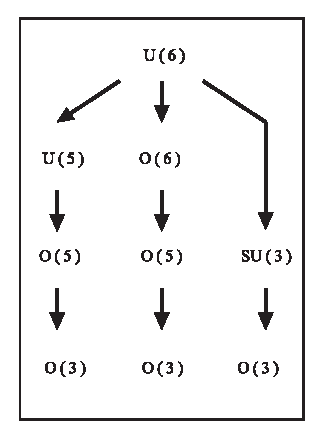
\includegraphics[height=4cm]{figure.eps}
%
% If not, use
%\picplace{5cm}{2cm} % Give the correct figure height and width in cm
%
\caption{Please write your figure caption here}
\label{fig:1}       % Give a unique label
\end{figure}
%
% For built-in environments use
%
\begin{theorem}
Theorem text goes here.
\end{theorem}
%
% or
%
\begin{lemma}
Lemma text goes here.
\end{lemma}
%
%
% Problems or Exercises should be sorted chapterwise
\section*{Problems}
\addcontentsline{toc}{section}{Problems}
%
% Use the following environment.
% Don't forget to label each problem;
% the label is needed for the solutions' environment
\begin{prob}
\label{prob1}
The problem\footnote{Footnote} is described here. The
problem is described here. The problem is described here.
\end{prob}

\begin{prob}
\label{prob2}
\textbf{Problem Heading}\\
(a) The first part of the problem is described here.\\
(b) The second part of the problem is described here.
\end{prob}



%

%%%%%%%%%%%%%%%%%%%%%% chapter.tex %%%%%%%%%%%%%%%%%%%%%%%%%%%%%%%%%
%
% sample chapter
%
% Use this file as a template for your own input.
%
%%%%%%%%%%%%%%%%%%%%%%%% Springer-Verlag %%%%%%%%%%%%%%%%%%%%%%%%%%

\chapter{Chapter Heading}
\label{intro} % Always give a unique label
% use \chaptermark{}
% to alter or adjust the chapter heading in the running head

Your text goes here. Separate text sections with the standard \LaTeX\
sectioning commands.

\section{Section Heading}
\label{sec:1}
% Always give a unique label
% and use \ref{<label>} for cross-references
% and \cite{<label>} for bibliographic references
% use \sectionmark{}
% to alter or adjust the section heading in the running head
Your text goes here. Use the \LaTeX\ automatism for your citations
\cite{monograph}.

\subsection{Subsection Heading}
\label{sec:2}
Your text goes here.

\begin{equation}
\vec{a}\times\vec{b}=\vec{c}
\end{equation}

\subsubsection{Subsubsection Heading}
Your text goes here. Use the \LaTeX\ automatism for cross-references as
well as for your citations, see Sect.~\ref{sec:1}.

\paragraph{Paragraph Heading} %
Your text goes here.

\subparagraph{Subparagraph Heading.} Your text goes here.%
%
\index{paragraph}
% Use the \index{} command to code your index words
%
% For tables use
%
\begin{table}
\centering
\caption{Please write your table caption here}
\label{tab:1}       % Give a unique label
%
% For LaTeX tables use
%
\begin{tabular}{lll}
\hline\noalign{\smallskip}
first & second & third  \\
\noalign{\smallskip}\hline\noalign{\smallskip}
number & number & number \\
number & number & number \\
\noalign{\smallskip}\hline
\end{tabular}
\end{table}
%
%
% For figures use
%
\begin{figure}
\centering
% Use the relevant command for your figure-insertion program
% to insert the figure file.
% For example, with the option graphics use
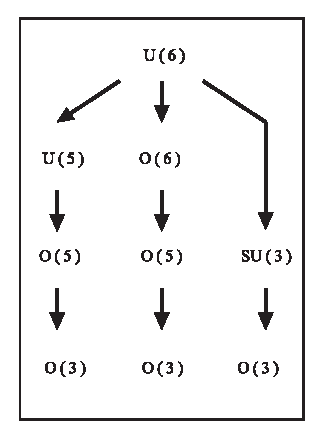
\includegraphics[height=4cm]{figure.eps}
%
% If not, use
%\picplace{5cm}{2cm} % Give the correct figure height and width in cm
%
\caption{Please write your figure caption here}
\label{fig:1}       % Give a unique label
\end{figure}
%
% For built-in environments use
%
\begin{theorem}
Theorem text goes here.
\end{theorem}
%
% or
%
\begin{lemma}
Lemma text goes here.
\end{lemma}
%
%
% Problems or Exercises should be sorted chapterwise
\section*{Problems}
\addcontentsline{toc}{section}{Problems}
%
% Use the following environment.
% Don't forget to label each problem;
% the label is needed for the solutions' environment
\begin{prob}
\label{prob1}
The problem\footnote{Footnote} is described here. The
problem is described here. The problem is described here.
\end{prob}

\begin{prob}
\label{prob2}
\textbf{Problem Heading}\\
(a) The first part of the problem is described here.\\
(b) The second part of the problem is described here.
\end{prob}



%

%\appendix
%%!TEX root = main.tex

\appendix
\onecolumn
\section*{Overview}
\begin{table}[H]
    \centering
    \hspace*{-1cm}\begin{tabular}{lllll}
    \toprule
    Name                     & Function $\varphi(x)$ & Range of Values & $\varphi'(x)$ & Used by \\\midrule % 
    Sign function$^\dagger$  & $\begin{cases}+1 &\text{if } x \geq 0\\-1 &\text{if } x < 0\end{cases}$ & $\Set{-1,1}$                              & $0$                    & \cite{971754} \\
    \parbox[t]{2.6cm}{Heaviside\\step function$^\dagger$} & $\begin{cases}+1 &\text{if } x > 0\\0 &\text{if } x < 0\end{cases}$ & $\Set{0, 1}$  & $0$                       & \cite{mcculloch1943logical}\\
    Logistic function        & $\frac{1}{1+e^{-x}}$                           & $[0, 1]$                                                        & $\frac{e^x}{(e^x +1)^2}$  & \cite{duch1999survey} \\
    Tanh                     & $\frac{e^x - e^{-x}}{e^x + e^{-x}} = \tanh(x)$ & $[-1, 1]$                                                       & $\sech^2(x)$              & \cite{LeNet-5,Thoma:2014}\\
    \gls{ReLU}$^\dagger$           & $\max(0, x)$                                   & $[0, +\infty)$                                                  & $\begin{cases}1 &\text{if } x > 0\\0 &\text{if } x < 0\end{cases}$      & \cite{AlexNet-2012}\\
    \parbox[t]{2.6cm}{\gls{LReLU}$^\dagger$\footnotemark\\(\gls{PReLU})} & $\varphi(x) = \max(\alpha x, x)$                        & $(-\infty, +\infty)$                                             & $\begin{cases}1 &\text{if } x > 0\\\alpha &\text{if } x < 0\end{cases}$ & \cite{maas2013rectifier,he2015delving} \\
    Softplus                 & $\log(e^x + 1)$                                & $(0, +\infty)$                                       & $\frac{e^x}{e^x + 1}$    & \cite{dugas2001incorporating,glorot2011deep} \\
    \gls{ELU}                & $\begin{cases}x &\text{if } x > 0\\\alpha (e^x - 1) &\text{if } x \leq 0\end{cases}$ & $(-\infty, +\infty)$ & $\begin{cases}1 &\text{if } x > 0\\\alpha e^x &\text{otherwise}\end{cases}$ & \cite{clevert2015fast} \\
    Softmax$^\ddagger$       & $o(\mathbf{x})_j = \frac{e^{x_j}}{\sum_{k=1}^K e^{x_k}}$    & $[0, 1]^K$                                           & $o(\mathbf{x})_j \cdot \frac{\sum_{k=1}^K e^{x_k} - e^{x_j}}{\sum_{k=1}^K e^{x_k}}$         & \cite{AlexNet-2012,Thoma:2014}\\
    Maxout$^\ddagger$        & $o(\mathbf{x}) = \max_{x \in \mathbf{x}} x$                 & $(-\infty, +\infty)$                                 & $\begin{cases}1 &\text{if } x_i = \max \mathbf{x}\\0 &\text{otherwise}\end{cases}$          & \cite{goodfellow2013maxout}       \\
    \bottomrule
    \end{tabular}
    \caption[Activation functions]{Overview of activation functions. Functions
             marked with $\dagger$ are not differentiable at 0 and functions
             marked with $\ddagger$ operate on all elements of a layer
             simultaneously. The hyperparameters $\alpha \in (0, 1)$ of Leaky
             ReLU and ELU are typically $\alpha = 0.01$. Other activation
             function like randomized leaky ReLUs exist~\cite{xu2015empirical},
             but are far less commonly used.\\
             Some functions are smoothed versions of others, like the logistic
             function for the Heaviside step function, tanh for the sign
             function, softplus for ReLU.\\
             Softmax is the standard activation function for the last layer of
             a classification network as it produces a probability
             distribution. See \Cref{fig:activation-functions-plot} for a plot
             of some of them.}
    \label{table:activation-functions-overview}
\end{table}
\footnotetext{$\alpha$ is a hyperparameter in leaky ReLU, but a learnable parameter in the parametric ReLU function.}

\section*{Evaluation Results}
\glsunset{LReLU}
\begin{table}[H]
    \centering
    \begin{tabular}{@{\extracolsep{4pt}}lcccccc@{}}
    \toprule
    \multirow{2}{*}{Function} & \multicolumn{4}{c}{Single model}                                                    & \multicolumn{2}{c}{Ensemble of 10} \\\cline{2-3}\cline{4-5}\cline{6-7}
                   & \multicolumn{2}{c}{Training set}     &\multicolumn{2}{c}{Test set}                  & Training set         & Test set \\\midrule
    Identity       & \SI{66.25}{\percent} & $\boldsymbol{\sigma=0.77}$ &\SI{56.74}{\percent} & \textbf{$\sigma=0.51$} & \SI{68.77}{\percent} & \SI{58.78}{\percent}\\
    Logistic       & \SI{51.87}{\percent} & $\sigma=3.64$ &\SI{46.54}{\percent} & $\sigma=3.22$          & \SI{61.19}{\percent} & \SI{54.58}{\percent}\\
    Logistic$^-$   & \SI{66.49}{\percent} & $\sigma=1.99$ &\SI{57.84}{\percent} & $\sigma=1.15$          & \SI{69.04}{\percent} & \SI{60.10}{\percent}\\
    Softmax        & \SI{75.22}{\percent} & $\sigma=2.41$ &\SI{59.49}{\percent} & $\sigma=1.25$          & \SI{78.87}{\percent} & \SI{63.06}{\percent}\\
    Tanh           & \SI{67.27}{\percent} & $\sigma=2.38$ &\SI{55.70}{\percent} & $\sigma=1.44$          & \SI{70.21}{\percent} & \SI{58.10}{\percent}\\
    Softsign       & \SI{66.43}{\percent} & $\sigma=1.74$ &\SI{55.75}{\percent} & $\sigma=0.93$          & \SI{69.78}{\percent} & \SI{58.40}{\percent}\\
    \gls{ReLU}     & \SI{78.62}{\percent} & $\sigma=2.15$ &\SI{62.18}{\percent} & $\sigma=0.99$          & \SI{81.81}{\percent} & \SI{64.57}{\percent}\\
    \gls{ReLU}$^-$ & \SI{76.01}{\percent} & $\sigma=2.31$ &\SI{62.87}{\percent} & $\sigma=1.08$          & \SI{78.18}{\percent} & \SI{64.81}{\percent}\\
    Softplus       & \SI{66.75}{\percent} & $\sigma=2.45$ &\SI{56.68}{\percent} & $\sigma=1.32$          & \SI{71.27}{\percent} & \SI{60.26}{\percent}\\
    S2ReLU         & \SI{63.32}{\percent} & $\sigma=1.69$ &\SI{56.99}{\percent} & $\sigma=1.14$          & \SI{65.80}{\percent} & \SI{59.20}{\percent}\\
    \gls{LReLU}    & \SI{74.92}{\percent} & $\sigma=2.49$ &\SI{61.86}{\percent} & $\sigma=1.23$          & \SI{77.67}{\percent} & \SI{64.01}{\percent}\\
    \gls{PReLU}    & \textbf{\SI{80.01}{\percent}} & $\sigma=2.03$ &\SI{62.16}{\percent} & $\sigma=0.73$ & \textbf{\SI{83.50}{\percent}} & \textbf{\SI{64.79}{\percent}}\\
    \gls{ELU}      & \SI{76.64}{\percent} & $\sigma=1.48$ &\textbf{\SI{63.38}{\percent}} & $\sigma=0.55$ & \SI{78.30}{\percent} & \SI{64.70}{\percent}\\
    \bottomrule
    \end{tabular}
    \caption[Activation function evaluation results on CIFAR-100]{Training and
             test accuracy of adjusted baseline models trained with different
             activation functions on CIFAR-100. For \gls{LReLU}, $\alpha = 0.3$ was
             chosen.}
    \label{table:CIFAR-100-accuracies-activation-functions}
\end{table}

\begin{table}[H]
    \centering
    \setlength\tabcolsep{1.5pt}
    \begin{tabular}{@{\extracolsep{4pt}}lcccccccr@{}}
    \toprule
    \multirow{2}{*}{Function} & \multicolumn{4}{c}{Single model}              & \multicolumn{2}{c}{Ensemble of 10} & \multicolumn{2}{c}{Epochs}\\\cline{2-5}\cline{6-7}\cline{8-9}
                              & \multicolumn{2}{c}{Training set}     &\multicolumn{2}{c}{Test set}                  & Train                & Test                 & Range     & \multicolumn{1}{c}{Mean} \\\midrule
    Identity                  & \SI{87.92}{\percent} & $\sigma=0.40$ & \SI{84.69}{\percent} & $\sigma=0.08$         & \SI{88.59}{\percent} & \SI{85.43}{\percent} & \hphantom{0}92 -- 140 & 114.5\\%TODO: Really?
    Logistic                  & \SI{81.46}{\percent} & $\sigma=5.08$ & \SI{79.67}{\percent} & $\sigma=4.85$         & \SI{86.38}{\percent} & \SI{84.60}{\percent} & \hphantom{0}\textbf{58} -- \hphantom{0}\textbf{91}  & \textbf{77.3}\\
    Softmax                   & \SI{88.19}{\percent} & $\sigma=0.31$ & \SI{84.70}{\percent} & $\sigma=0.15$         & \SI{88.69}{\percent} & \SI{85.43}{\percent} & 124 -- 171& 145.8\\
    Tanh                      & \SI{88.41}{\percent} & $\sigma=0.36$ & \SI{84.46}{\percent} & $\sigma=0.27$         & \SI{89.24}{\percent} & \SI{85.45}{\percent} & \hphantom{0}89 -- 123 & 108.7\\
    Softsign                  & \SI{88.00}{\percent} & $\sigma=0.47$ & \SI{84.46}{\percent} & $\sigma=0.23$         & \SI{88.77}{\percent} & \SI{85.33}{\percent} & \hphantom{0}77 -- 119 & 104.1\\
    \gls{ReLU}                & \SI{88.93}{\percent} & $\sigma=0.46$ & \textbf{\SI{85.35}{\percent}} & $\sigma=0.21$         & \SI{89.35}{\percent} & \SI{85.95}{\percent} & \hphantom{0}96 -- 132 & 102.8\\
    Softplus                  & \SI{88.42}{\percent} & $\boldsymbol{\sigma=0.29}$ & \SI{85.16}{\percent} & $\sigma=0.15$         & \SI{88.90}{\percent} & \SI{85.73}{\percent} &            108 -- 143 & 121.0\\
    \gls{LReLU}               & \SI{88.61}{\percent} & $\sigma=0.41$ & \SI{85.21}{\percent} & $\boldsymbol{\sigma=0.05}$         & \SI{89.07}{\percent} & \SI{85.83}{\percent} & \hphantom{0}87 -- 117 & 104.5\\
    \gls{PReLU}               & \textbf{\SI{89.62}{\percent}} & $\sigma=0.41$ & \textbf{\SI{85.35}{\percent}} & $\sigma=0.17$& \textbf{\SI{90.10}{\percent}} & \SI{86.01}{\percent} & \hphantom{0}85 -- 111 & 100.5\\
    \gls{ELU}                 & \SI{89.49}{\percent} & $\sigma=0.42$ & \textbf{\SI{85.35}{\percent}} & $\sigma=0.10$         & \SI{89.94}{\percent} & \textbf{\SI{86.03}{\percent}} & \hphantom{0}73 -- 113 &  92.4\\
    \bottomrule
    \end{tabular}
    \caption[Activation function evaluation results on HASYv2]{Test accuracy of
             adjusted baseline models trained with different activation
             functions on HASYv2. For \gls{LReLU}, $\alpha = 0.3$ was chosen.}
    \label{table:HASYv2-accuracies-activation-functions}
\end{table}

\begin{table}[H]
    \centering
    \setlength\tabcolsep{1.5pt}
    \begin{tabular}{@{\extracolsep{4pt}}lcccccccr@{}}
    \toprule
    \multirow{2}{*}{Function} & \multicolumn{4}{c}{Single model}              & \multicolumn{2}{c}{Ensemble of 10} & \multicolumn{2}{c}{Epochs}\\\cline{2-5}\cline{6-7}\cline{8-9}
                              & \multicolumn{2}{c}{Training set}     &\multicolumn{2}{c}{Test set}                  & Train                & Test                 & Range     & \multicolumn{1}{c}{Mean} \\\midrule
    Identity                  & \SI{87.49}{\percent} & $\sigma=2.50$ & \SI{69.86}{\percent} & $\sigma=1.41$         & \SI{89.78}{\percent} & \SI{71.90}{\percent} & \hphantom{0}51 -- \hphantom{0}65  &  53.4\\
    Logistic                  & \SI{45.32}{\percent} & $\sigma=14.88$& \SI{40.85}{\percent} & $\sigma=12.56$        & \SI{51.06}{\percent} & \SI{45.49}{\percent} & \hphantom{0}38 -- \hphantom{0}93  &  74.6\\
    Softmax                   & \SI{87.90}{\percent} & $\sigma=3.58$ & \SI{67.91}{\percent} & $\sigma=2.32$         & \SI{91.51}{\percent} & \SI{70.96}{\percent} & 108 -- 150           & 127.5\\
    Tanh                      & \SI{85.38}{\percent} & $\sigma=4.04$ & \SI{67.65}{\percent} & $\sigma=2.01$         & \SI{90.47}{\percent} & \SI{71.29}{\percent} & 48 -- \hphantom{0}92 & 65.2\\
    Softsign                  & \SI{88.57}{\percent} & $\sigma=4.00$ & \SI{69.32}{\percent} & $\sigma=1.68$         & \SI{93.04}{\percent} & \SI{72.40}{\percent} & 55 -- 117            & 83.2\\
    \gls{ReLU}                & \SI{94.35}{\percent} & $\sigma=3.38$ & \SI{71.01}{\percent} & $\sigma=1.63$         & \SI{98.20}{\percent} & \SI{74.85}{\percent} & 52 -- \hphantom{0}98 & 75.5\\
    Softplus                  & \SI{83.03}{\percent} & $\sigma=2.07$ & \SI{68.28}{\percent} & $\sigma=1.74$         & \SI{93.04}{\percent} & \SI{75.99}{\percent} & 56 -- \hphantom{0}89 & 68.9\\
    \gls{LReLU}               & \SI{93.83}{\percent} & $\sigma=3.89$ & \SI{74.66}{\percent} & $\sigma=2.11$         & \SI{97.56}{\percent} & \SI{78.08}{\percent} & 52 -- 120 & 80.1\\
    \gls{PReLU}               & \SI{95.53}{\percent} & $\sigma=1.92$ & \SI{71.69}{\percent} & $\sigma=1.37$         & \SI{98.17}{\percent} & \SI{74.69}{\percent} & 59 -- 101 & 78.8\\
    \gls{ELU}                 & \SI{95.42}{\percent} & $\sigma=3.57$ & \SI{75.09}{\percent} & $\sigma=2.39$         & \SI{98.54}{\percent} & \SI{78.66}{\percent} & 66 -- \hphantom{0}72 & 67.2\\
    \bottomrule
    \end{tabular}
    \caption[Activation function evaluation results on STL-10]{Test accuracy of
             adjusted baseline models trained with different activation
             functions on STL-10. For \gls{LReLU}, $\alpha = 0.3$ was chosen.}
    \label{table:STL-10-accuracies-activation-functions}
\end{table}

\begin{table}[H]
    \centering
    \hspace*{-1cm}\begin{tabular}{lllll}
    \toprule
    Name                     & Function $\varphi(x)$ & Range of Values & $\varphi'(x)$ \\\midrule % & Used by 
    Sign function$^\dagger$  & $\begin{cases}+1 &\text{if } x \geq 0\\-1 &\text{if } x < 0\end{cases}$ & $\Set{-1,1}$                              & $0$                    \\%& \cite{971754} \\
    \parbox[t]{2.6cm}{Heaviside\\step function$^\dagger$} & $\begin{cases}+1 &\text{if } x > 0\\0 &\text{if } x < 0\end{cases}$ & $\Set{0, 1}$  & $0$                       \\%& \cite{mcculloch1943logical}\\
    Logistic function        & $\frac{1}{1+e^{-x}}$                           & $[0, 1]$                                                        & $\frac{e^x}{(e^x +1)^2}$  \\%& \cite{duch1999survey} \\
    Tanh                     & $\frac{e^x - e^{-x}}{e^x + e^{-x}} = \tanh(x)$ & $[-1, 1]$                                                       & $\sech^2(x)$              \\%& \cite{LeNet-5,Thoma:2014}\\
    \gls{ReLU}$^\dagger$           & $\max(0, x)$                                   & $[0, +\infty)$                                                  & $\begin{cases}1 &\text{if } x > 0\\0 &\text{if } x < 0\end{cases}$      \\%& \cite{AlexNet-2012}\\
    \parbox[t]{2.6cm}{\gls{LReLU}$^\dagger$\footnotemark\\(\gls{PReLU})} & $\varphi(x) = \max(\alpha x, x)$                        & $(-\infty, +\infty)$                                             & $\begin{cases}1 &\text{if } x > 0\\\alpha &\text{if } x < 0\end{cases}$ \\%& \cite{maas2013rectifier,he2015delving} \\
    Softplus                 & $\log(e^x + 1)$                                & $(0, +\infty)$                                       & $\frac{e^x}{e^x + 1}$    \\%& \cite{dugas2001incorporating,glorot2011deep} \\
    \gls{ELU}                & $\begin{cases}x &\text{if } x > 0\\\alpha (e^x - 1) &\text{if } x \leq 0\end{cases}$ & $(-\infty, +\infty)$ & $\begin{cases}1 &\text{if } x > 0\\\alpha e^x &\text{otherwise}\end{cases}$ \\%& \cite{clevert2015fast} \\
    Softmax$^\ddagger$       & $o(\mathbf{x})_j = \frac{e^{x_j}}{\sum_{k=1}^K e^{x_k}}$    & $[0, 1]^K$                                           & $o(\mathbf{x})_j \cdot \frac{\sum_{k=1}^K e^{x_k} - e^{x_j}}{\sum_{k=1}^K e^{x_k}}$          \\%& \cite{AlexNet-2012,Thoma:2014}\\
    Maxout$^\ddagger$        & $o(\mathbf{x}) = \max_{x \in \mathbf{x}} x$                 & $(-\infty, +\infty)$                                 & $\begin{cases}1 &\text{if } x_i = \max \mathbf{x}\\0 &\text{otherwise}\end{cases}$          \\%& \cite{goodfellow2013maxout}       \\
    \bottomrule
    \end{tabular}
    \caption[Activation functions]{Overview of activation functions. Functions
             marked with $\dagger$ are not differentiable at 0 and functions
             marked with $\ddagger$ operate on all elements of a layer
             simultaneously. The hyperparameters $\alpha \in (0, 1)$ of Leaky
             ReLU and ELU are typically $\alpha = 0.01$. Other activation
             function like randomized leaky ReLUs exist~\cite{xu2015empirical},
             but are far less commonly used.\\
             Some functions are smoothed versions of others, like the logistic
             function for the Heaviside step function, tanh for the sign
             function, softplus for ReLU.\\
             Softmax is the standard activation function for the last layer of
             a classification network as it produces a probability
             distribution. See \Cref{fig:activation-functions-plot} for a plot
             of some of them.}
    \label{table:activation-functions-overview}
\end{table}
\footnotetext{$\alpha$ is a hyperparameter in leaky ReLU, but a learnable parameter in the parametric ReLU function.}

\begin{figure}[ht]
    \centering
    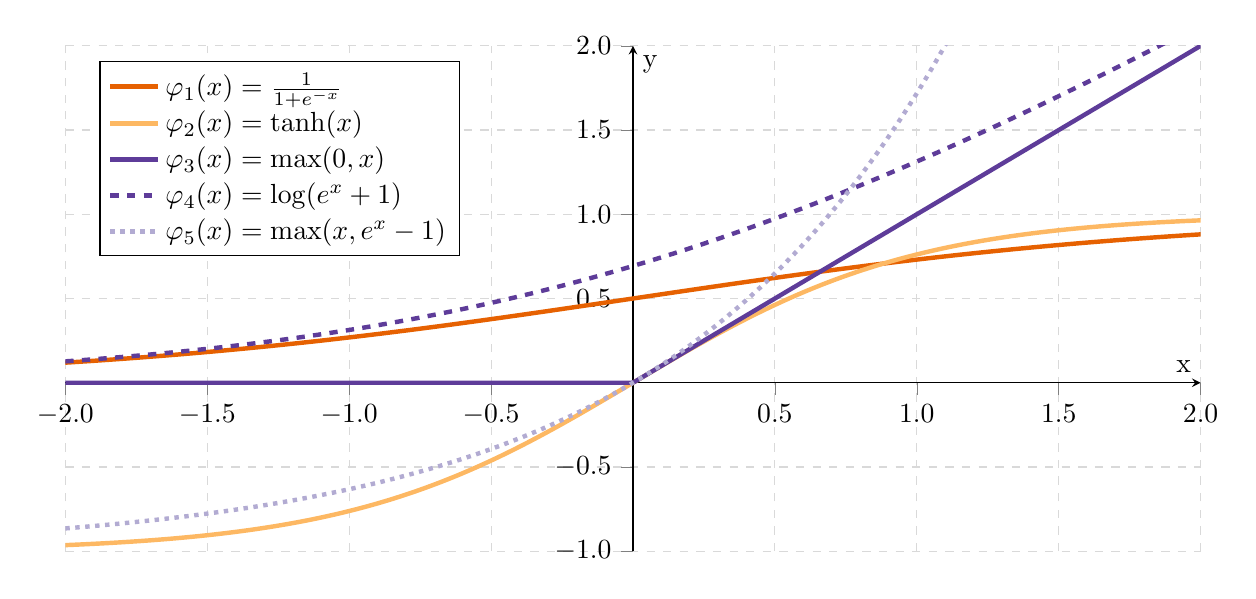
\begin{tikzpicture}
        \definecolor{color1}{HTML}{E66101}
        \definecolor{color2}{HTML}{FDB863}
        \definecolor{color3}{HTML}{B2ABD2}
        \definecolor{color4}{HTML}{5E3C99}
        \begin{axis}[
            legend pos=north west,
            legend cell align={left},
            axis x line=middle,
            axis y line=middle,
            x tick label style={/pgf/number format/fixed,
                                /pgf/number format/fixed zerofill,
                                /pgf/number format/precision=1},
            y tick label style={/pgf/number format/fixed,
                                /pgf/number format/fixed zerofill,
                                /pgf/number format/precision=1},
            grid = major,
            width=16cm,
            height=8cm,
            grid style={dashed, gray!30},
            xmin=-2,     % start the diagram at this x-coordinate
            xmax= 2,     % end   the diagram at this x-coordinate
            ymin=-1,     % start the diagram at this y-coordinate
            ymax= 2,     % end   the diagram at this y-coordinate
            xlabel=x,
            ylabel=y,
            tick align=outside,
            enlargelimits=false]
          \addplot[domain=-2:2, color1, ultra thick,samples=500] {1/(1+exp(-x))};
          \addplot[domain=-2:2, color2, ultra thick,samples=500] {tanh(x)};
          \addplot[domain=-2:2, color4, ultra thick,samples=500] {max(0, x)};
          \addplot[domain=-2:2, color4, ultra thick,samples=500, dashed] {ln(exp(x) + 1)};
          \addplot[domain=-2:2, color3, ultra thick,samples=500, dotted] {max(x, exp(x) - 1)};
          \addlegendentry{$\varphi_1(x)=\frac{1}{1+e^{-x}}$}
          \addlegendentry{$\varphi_2(x)=\tanh(x)$}
          \addlegendentry{$\varphi_3(x)=\max(0, x)$}
          \addlegendentry{$\varphi_4(x)=\log(e^x + 1)$}
          \addlegendentry{$\varphi_5(x)=\max(x, e^x - 1)$}
        \end{axis}
    \end{tikzpicture}
    \caption[Activation functions]{Activation functions plotted in $[-2, +2]$.
             $\tanh$ and ELU are able to produce negative numbers. The image of
             ELU, ReLU and Softplus is not bound on the positive side, whereas
             $\tanh$ and the logistic function are always below~1.}
    \label{fig:activation-functions-plot}
\end{figure}

\glsreset{LReLU}
\twocolumn

\backmatter%%%%%%%%%%%%%%%%%%%%%%%%%%%%%%%%%%%%%%%%%%%%%%%%%%%%%%%

\chapter*{Solutions}
\addcontentsline{toc}{chapter}{Solutions}
\markboth{Solutions}{Solutions}

\section*{Problems of Chapter~\ref{intro}}

\begin{sol}{prob1}
The solution is revealed here.
\end{sol}


\begin{sol}{prob2}
\textbf{Problem Heading}\\
(a) The solution of first part is revealed here.\\
(b) The solution of second part is revealed here.
\end{sol}


%%%%%%%%%%%%%%%%%%%%%%%% referenc.tex %%%%%%%%%%%%%%%%%%%%%%%%%%%%%%
% sample references
% "computer science"
%
% Use this file as a template for your own input.
%
%%%%%%%%%%%%%%%%%%%%%%%% Springer-Verlag %%%%%%%%%%%%%%%%%%%%%%%%%%

%
% BibTeX users please use
% \bibliographystyle{}
% \bibliography{}
%
% Non-BibTeX users please use
\begin{thebibliography}{99.}
%
% and use \bibitem to create references.
%
% Use the following syntax and markup for your references
%
% Monographs
\bibitem{monograph} Kajan E (2002)
Information technology encyclopedia and acronyms. Springer, Berlin
Heidelberg New York

% Contributed Works
\bibitem{contribution} Broy M (2002) Software engineering -- From
auxiliary to key technologies. In: Broy M, Denert E (eds)
Software Pioneers. Springer, Berlin Heidelberg New York

% Journal
\bibitem{journal} Che M, Grellmann W, Seidler S (1997)
Appl Polym Sci 64:1079--1090

% Theses
\bibitem{thesis} Ross DW (1977) Lysosomes and storage diseases. MA
Thesis, Columbia University, New York

\end{thebibliography}

\printindex

%%%%%%%%%%%%%%%%%%%%%%%%%%%%%%%%%%%%%%%%%%%%%%%%%%%%%%%%%%%%%%%%%%%%%%

\end{document}





